\section{Motivation}
Die Motivation dieses Versuchs besteht in der Bestimmung der Planckkonstante mithilfe des Fotoeffekts.
Die Plackkonstante ist eine fundamentale Größe in der Quantenphysik und kennzeichnet die
Quantisierung der Energie. Für die Bestimmung eignet sich der Fotoeffekt,
da dieser eine anschauliche Möglichkeit bietet die Quantisierung des Lichts zu verstehen.


\section{Messverfahren}

Das Licht einer Hg-Dampflampe wird durch einen Kollimator zu einem Doppelprisma geschickt.
Durch den Kollimator sind die Strahlen parallel, weshalb das Licht am Doppelprisma in sein Spektrum zerlegt wird.
Anschließend wird das Licht in einen Kasten gespiegelt. In dem Kasten befindet sich ein Papierschirm,
auf den das Licht mittels eines Hebels umgelenkt werden kann um die gewünschte Spektrallinie zu finden.
Anschließend wird der Hebel umgelegt und mit dem Multimeter das Maximum der messbaren Spannung gesucht.
Dann wird die Vorspannung in $100$ mV Schritten heruntergesetzt und jeweils der Fotostrom mithilfe des Multimeters gemessen.
Der Fotostrom wird mit durch einen Spannungswandler als Spannung abgelesen.
\begin{figure}[h!]
    \centering
    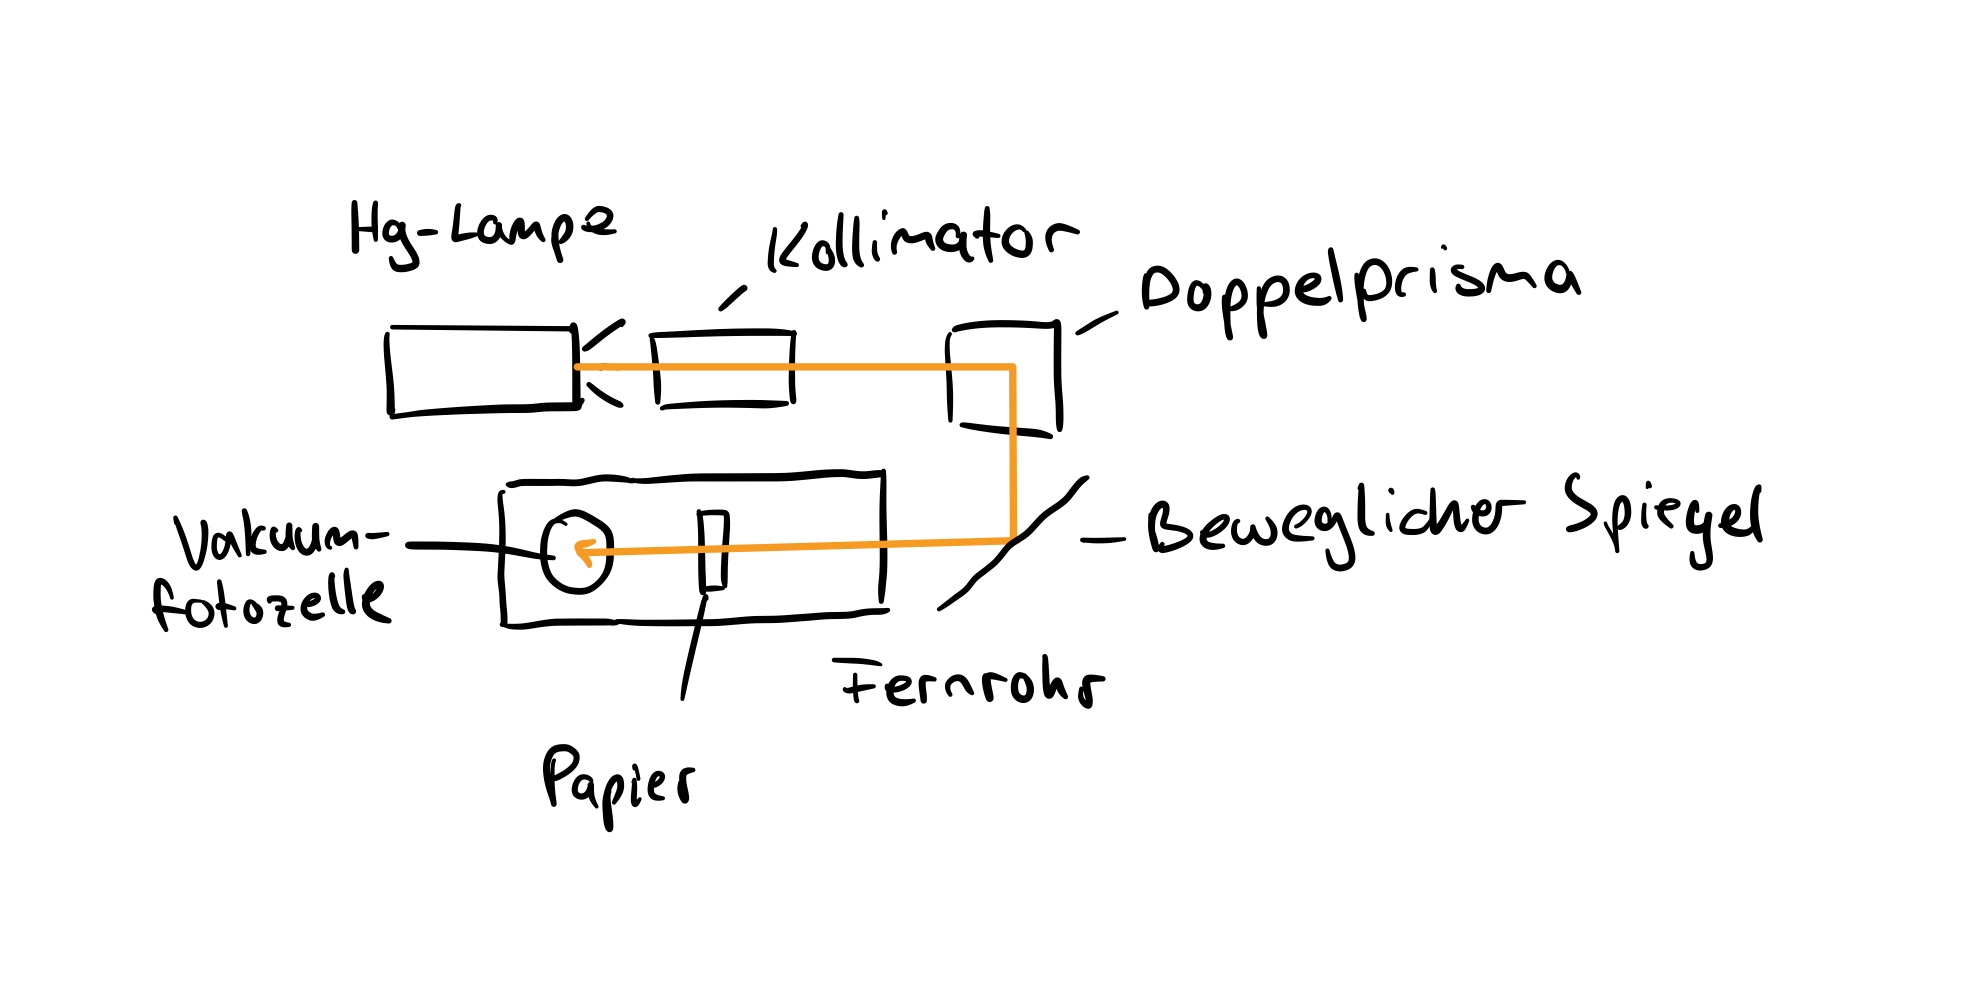
\includegraphics[width=0.9\textwidth,]{35-Skizze.jpeg}
    \caption{Aufbauskizze}
\end{figure}
\section{Grundlagen aus der Physik}
\subsection{Fotozelle}

Die Photozelle besteht aus einer Kathode, auf welche das Licht einfällt, und eine Ringanode, welche die austretenden Elektronen
aufnehmen soll. Die Fotokathode besteht aus bedampftem Kalium welches eine deutlich geringere Austrittsarbeit hat, als das
Kupfer aus dem die Anode besteht. Das sorgt dafür, dass aus der Anode möglichst keine Elektronen austreten.
Der Elektronenfluss zwischen Fotokathode und Ringanode kann mittels eines Multimeters abgelesen werden.
Diese Ströme sind sehr klein, weshalb sie mit einem Spannungswandler verstärkt werden.

\subsection{Energieverteilung von Elektronen in Metall}

In einem Metall bilden die Atome ein Metallgitter, was dafür sorgt,dass sich die Valenzelektronen innerhalb des Metalls
nahezu frei bewegen können. Diese werden als Leitungselektronen bezeichnet. Sie können das Metall nciht ohne weiteres verlassen,
da sie von den Atomkernen immer noch angezogen werden.\\
Die Energieverteilung dieser Elektronen unterliegt der sog Fermiverteilung.
Diese besagt, dass bei $T= 0K$ alle Energiezustände bis zu einer Maximalenergie, der Fermienergie $E_F$,
besetzt sind. Zustände über dieser Energie treten nicht auf.\\
Bei Temperaturen über $0K$ ``verschwimmt'' die Grenze der Fermienergie. Das heißt, das auch Zunstände
über dieser Energie auftreten.\\
Ein Metall hat eine charakteristische Austrittsarbeit $A$, welche über die Fermienergie hinaus geleistet werden muss um das Elektron in den Außenraum zu bewegen.
Trifft nun ein Photon mit der Energie $h \nu$ ein Leitungselektron mit der Energie $E_e$ wird die Energie auf das Elektron übertragen.
Ist diese Energie groß genug kann das Elektron das Metall verlassen. Für die benötigte Energie gilt:
\begin{equation}
    h \nu =  A + (E_F - E_e) + E_{kin}
\end{equation}
Für die maximale Energie eines Elektrons gilt, dass es sich bei der Fermienergie befindet. Dieserr Fall ist bei Temperaturen über 0 K
nicht immer gegeben. Legt man nun eine Spannung $U$ so an, dass die die Elektronen bremst, gibt es im Idealfall eine Spannung $U_s$ bei der kein
Strom mehr fließt. Da dies nur den Idealfall betrifft und es Elektronen gibt die es trotz $U> U_i$ zur Anode schaffen muss der Fall für Spannungen unter
$U_s$ asymptotisch angenähert werden. Die Nullstelle dieser geraden entspricht der theoretischen Sperrspannung $U_s$.
\begin{equation}
    E_{kin,\max}= h \nu - A
    \label{eq:Ekin}
\end{equation}

\textbf{Elektronen im elektrischen Feld} besitzen die Energie $E = e U$ welche bei der Sperrspannung genau der kinetischen Energie der Elektronen entsprechen muss, da kein Strom fließt.
Mit $e$ als Elementarladung und $U$ als angelegte Spannung.
Daraus folgt mit Gleichung \ref{eq:Ekin}:
\begin{equation}
    eU_s = h \nu - A
\end{equation}
\begin{equation}
    \Rightarrow\frac{d U_s (\nu)}{d \nu} = \frac{h}{e}
    \label{eq:hfertig}
\end{equation}

Durch den Spannungswandler wird am Multimeter eine Spannung $U_I$ gemessen, welche nach dem Ohmschen Gesetz proportional zu Spannung ist.
Da unserer Messaufbau für einen Untergrundsstrom $U_i0$ sorgt muss dieser zuerst eliminiert werden. Dies führt zu de folgenden Relation:

\begin{equation}
    I \propto U_I - U_{I0}
\end{equation}
Die Geometrie der Fotozelle sorgt für einen Zusammenhang zwischen gemessenem Strom $I$ und Gegenspannung $U$von:
\begin{equation}
    U \propto \sqrt{I} 
\end{equation}
Setzt man diese beiden Zusammenhänge zusammen erhält man:
\begin{equation}
    U \propto \sqrt{U_I - U_{I0}} 
\end{equation}

Deshalb wird in den folgenden Diagrammen die Gegenspannung $U$ gegen $\sqrt{U_I - U_{I0}}$ aufgetragen.

\section{Standartabweichung}
Allgemein lässt sich die Abweichung eines Messwertes $x$ zu einem Literaturwert $x_{Lit}$ darstellen durch die Sigmaabweichung:

\begin{equation}
    \frac{|x-x_{Lit}|}{\Delta x} = k \sigma \ \ mit \ k \in \mathbb{R}
    \label{eq:sigma}
\end{equation}
